% --- IMPORTS ---
\documentclass[leqno]{article}
\usepackage{graphicx}
\usepackage{dsfont}
\usepackage{mathtools}
\usepackage{amssymb}
\usepackage{amsmath}
\usepackage{amsthm}
\usepackage{float}
\usepackage{ragged2e}
\usepackage{tensor}
\usepackage{fancyhdr}
\usepackage{empheq}
\usepackage[most]{tcolorbox}
\usepackage{enumitem}
\usepackage{dirtytalk}
\usepackage{marginnote}
\usepackage{microtype}
\usepackage[
  a4paper,
  left=0.8in,
  right=1in,
  top=1in,
  bottom=0.5in,
  headheight=14pt,
  headsep=0.4in
]{geometry}
\setlength{\parindent}{0cm}
% --- TikZ Packages ---
\usepackage{pgfplots}
\pgfplotsset{compat=1.18}
\usepgfplotslibrary{fillbetween, polar}
\usetikzlibrary{calc, positioning}
\usetikzlibrary{angles, quotes}
\usetikzlibrary{arrows.meta}
\usetikzlibrary{decorations.pathreplacing, decorations.markings}
\usetikzlibrary{patterns}
\usetikzlibrary{intersections}
% --- URL Packages ---
\usepackage[colorlinks=true,linkcolor=red,citecolor=magenta,urlcolor=black]{hyperref}%
\urlstyle{same}
% --- END OF IMPORTS ---

% --- CUSTOM COMMANDS ---
\RenewDocumentCommand{\marks}{o m}{%
  \IfValueTF{#1}%
    {\marginnote{\raggedright\textbf{[#2]}}[#1]}%
    {\marginnote{\raggedright\textbf{[#2]}}}%
}
\newcommand{\vspacerule}[2]{%
  \par\vspace*{#1}%
  \noindent\hrulefill\par
  \vspace*{#2}%
}
\definecolor{scarlet}{RGB}{205, 40, 75}
\newcommand{\questionitem}{%
  \item\phantomsection
  \addcontentsline{toc}{section}{Question \number\value{enumi}}%
}
\renewcommand{\contentsname}{Questions}
% --- END OF CUSTOM COMMANDS ---

% --- HEADER CONFIG ---
\pagestyle{fancy}
\fancyhead{}
\fancyfoot{}
\renewcommand{\headrulewidth}{0.9pt}
\lhead{Loci and Regions in the Argand Diagram}
\chead{}
\rhead{\href{https://danieljsmith.org}{danieljsmith.org}}
% --- END OF HEADER CONFIG ---

\begin{document}
\vspace*{20pt}
\tableofcontents
\newpage
\begin{enumerate}[
  label=\textbf{\arabic*.},
  leftmargin=*,
  topsep=0pt,
  partopsep=0pt,
  parsep=0pt
]

% ---- Question 1 ----
\questionitem
% [Source: _QBT__Loci_and_Regions_in_the_Argand_Diagram, Q1]

\begin{figure}[H]
    \centering
\begin{tikzpicture}[scale=0.75]
\def\cx{-2}
\def\cy{1}
\def\rad{4}

\coordinate (C) at (\cx,\cy);

\draw[-{Stealth[length=3mm]}, thick] (-6.3,0) -- (4.7,0) node[right] {$\mathrm{Re}(z)$};
\draw[-{Stealth[length=3mm]}, thick] (0,-4.3) -- (0,6.3) node[above] {$\mathrm{Im}(z)$};

\draw[thick] (C) circle (\rad);

\draw[thick] (\cx,0.12) -- (\cx,-0.12);
\draw[thick] (0.12,\cy) -- (-0.12,\cy);

\node[below left] at (0,0) {$O$};
\node[below] at (\cx,0) {$-2$};
\node[left] at (0,\cy) {$1$};
\end{tikzpicture}
\end{figure}


The Argand diagram shows a circle of radius $4$. The centre of the circle is the point which represents the complex number $-2+\mathrm{i}$. \\

\begin{enumerate}[label=\textbf{(\alph*)}]
  \item Use set notation to define the locus of complex numbers, $z$, represented by points which lie on the circle. \marks{2} \\
\end{enumerate}

The locus $L$ is defined by
\[
L=\Bigl\{z\in\mathbb{C}\;\Bigm|\; |z-(-2+\mathrm{i})|=|z+1-3\mathrm{i}|\Bigr\}
\] \\

\begin{enumerate}[label=\textbf{(\alph*)}, resume]
  \item On a copy of the Argand diagram, sketch and label the locus $L$. \marks{2} \\
\end{enumerate}

You are given that the locus
\[
\Bigl\{z\in\mathbb{C}\;\Bigm|\; \arg(z+1-2\mathrm{i})=\frac{2\pi}{3},\ \mathrm{Im}(z)=5\Bigr\}
\]
contains only one number. \\

\begin{enumerate}[label=\textbf{(\alph*)}, resume]
  \item Find this number. \marks{2} \\
\end{enumerate}

\newpage

% ---- Question 2 ----
\questionitem
% [Source: _QBT__Loci_and_Regions_in_the_Argand_Diagram, Q2]

In an Argand diagram, the point $P$ representing the complex number $w$ lies on the locus defined by \[\Bigl\{ z\in\mathbb{C}\;\Bigm|\; \arg(z-2+\mathrm{i})=\frac{\pi}{6} \Bigr\}\] You are given that $\mathrm{Im}(w)=3$. \\

\begin{enumerate}[label=\textbf{(\alph*)}]
  \item Find $w$. \marks{2} \\
\end{enumerate}

The point $P$ also lies on the locus defined by $\Bigl\{ z\in\mathbb{C}\;\Bigm|\; \lvert z-2-11\mathrm{i}\rvert =k \Bigr\}$, where $k$ is a constant. \\

\begin{enumerate}[label=\textbf{(\alph*)}, resume]
  \item Find the complex number represented by the other point of intersection of the loci defined by \[\Bigl\{ z\in\mathbb{C}\;\Bigm|\; \lvert z-2-11\mathrm{i}\rvert =k \Bigr\}\quad\text{and}\quad\Bigl\{ z\in\mathbb{C}\;\Bigm|\; \arg(z-2+\mathrm{i})=\frac{\pi}{6} \Bigr\}\] \marks{7} \\
\end{enumerate}

\newpage

% ---- Question 3 ----
\questionitem
% [Source: _QBT__Loci_and_Regions_in_the_Argand_Diagram, Q3]

On an Argand diagram, the locus of points satisfying $|z-4+3\mathrm{i}|=8$ is a circle. \\

\begin{enumerate}[label=\textbf{(\alph*)}]
  \item Write down
  \begin{enumerate}[label=(\roman*)]
    \item the coordinates of the centre of this circle \marks{1}
    \item the radius of this circle \marks{1}
  \end{enumerate}
  \item On an Argand diagram, shade the set of points defined by
  \[
  |z-4+3\mathrm{i}|\le 8
  \]
  \marks[-20pt]{1}
  \item For the set of points defined in part (b), determine the maximum value of $|z|$. \marks{3} \\
\end{enumerate}

The set of points $A$ is defined by
\[
A=
\Bigl\{ z\in\mathbb{C}\;\Bigm|\; -\frac{\pi}{4}\le \arg(z-3-6\mathrm{i})\le \frac{3\pi}{4} \Bigr\}
\mathbin{\textstyle\bigcap}
\Bigl\{ z\in\mathbb{C}\;\Bigm|\; \lvert z-4+3\mathrm{i}\rvert \le 8 \Bigr\}
\]

\begin{enumerate}[label=\textbf{(\alph*)}, resume]
  \item Determine the area of the region defined by $A$, giving your answer to 3 significant figures. \marks{4} \\
\end{enumerate}

\newpage

% ---- Question 4 ----
\questionitem
% [Source: _QBT__Loci_and_Regions_in_the_Argand_Diagram, Q4]

\begin{figure}[H]
    \centering
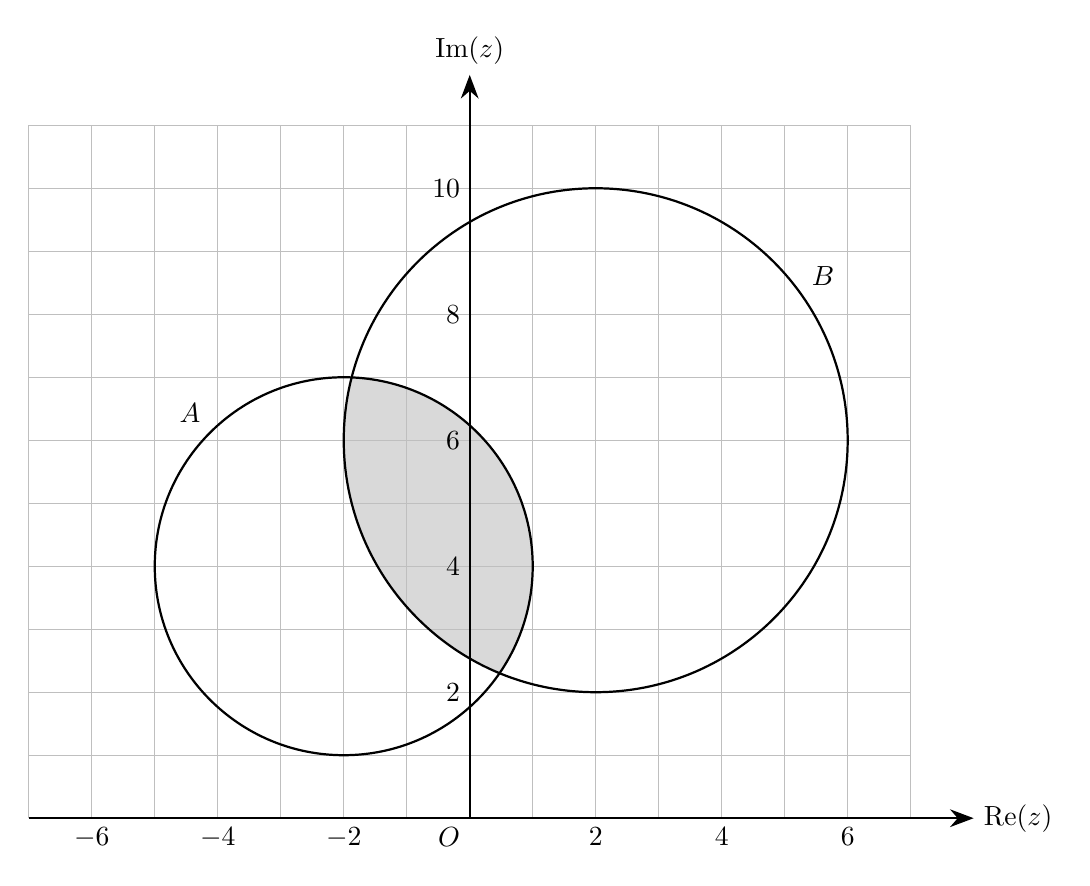
\begin{tikzpicture}[scale=0.8]
\def\xmin{-7}
\def\xmax{7}
\def\ymin{0}
\def\ymax{11}
\def\XA{-2}
\def\YA{4}
\def\RA{3}
\def\XB{2}
\def\YB{6}
\def\RB{4}

\coordinate (Ac) at (\XA,\YA);
\coordinate (Bc) at (\XB,\YB);

\begin{scope}
  \clip (Ac) circle (\RA);
  \fill[gray!30] (Bc) circle (\RB);
\end{scope}

\draw[gray!50, very thin] (\xmin,\ymin) grid (\xmax,\ymax);

\draw[thick] (Ac) circle (\RA);
\draw[thick] (Bc) circle (\RB);

\draw[-{Stealth[length=3mm]}, thick] (\xmin,0) -- (\xmax+1.0,0) node[right] {$\mathrm{Re}(z)$};
\draw[-{Stealth[length=3mm]}, thick] (0,\ymin) -- (0,\ymax+0.8) node[above] {$\mathrm{Im}(z)$};

\foreach \x in {-6,-4,-2,2,4,6} {
  \node[below] at (\x,0) {$\x$};
}
\foreach \y in {2,4,6,8,10} {
  \node[left] at (0,\y) {$\y$};
}
\node[below left] at (0,0) {$O$};

\node[above left] at ($(Ac)+(135:\RA)$) {$A$};
\node[above right] at ($(Bc)+(35:\RB)$) {$B$};
\end{tikzpicture}
\end{figure}


\begin{enumerate}[label=\textbf{(\alph*)}]
  \item The diagram above shows an Argand diagram.
  \begin{enumerate}[label=(\roman*)]
    \item Write down the equation of the locus represented by the circumference of circle $A$. \marks{3}
    \item Write down the two inequalities that define the shaded region, not including either circumference. \marks{3} \\
  \end{enumerate}
  \item
  \begin{enumerate}[label=(\roman*)]
    \item Draw an Argand diagram to show the region where
    \[
    -\frac{\pi}{6}<\arg\bigl(z+2-\mathrm{i}\bigr)<\frac{\pi}{4}
    \]
    \marks[-20pt]{3}
    \item Determine whether the point $1+5\mathrm{i}$ lies within this region. \marks{3} \\
  \end{enumerate}
\end{enumerate}

\newpage

% ---- Question 5 ----
\questionitem
% [Source: _QBT__Loci_and_Regions_in_the_Argand_Diagram, Q5]

\begin{figure}[H]
    \centering
\begin{tikzpicture}[scale=1]
\coordinate (O) at (0,0);
\draw[thick, -{Stealth[length=3mm]}] (-2.8,0) -- (6.8,0) node[right] {$\mathrm{Re}(z)$};
\draw[thick, -{Stealth[length=3mm]}] (0,-5.8) -- (0,3.8) node[above] {$\mathrm{Im}(z)$};
\node[below left] at (O) {$O$};
\end{tikzpicture}
\end{figure}


\begin{enumerate}[label=\textbf{(\alph*)}]
  \item Find the modulus of the complex number $2+2\sqrt{3}\mathrm{i}$, giving your answer as an integer. \marks{2} \\
  \item The locus of points, $L$, satisfies the equation $|z-(2-2\sqrt{3}\mathrm{i})|=2$.
  \begin{enumerate}[label=(\roman*)]
    \item Sketch the locus $L$ on the Argand diagram below. \marks{3}
    \item The complex number $w$ lies on $L$ so that $-\pi<\arg w\leq \pi$. Find the greatest possible value of $\arg w$, giving your answer in terms of $\pi$. \marks{2} \\
  \end{enumerate}
  \item Solve the equation $z^4=2+2\sqrt{3}\mathrm{i}$, giving your answers in the form $re^{\mathrm{i}\theta}$, where $r>0$ and $-\pi<\theta\leq \pi$. \marks{5} \\
\end{enumerate}

\newpage

% ---- Question 6 ----
\questionitem
% [Source: _QBT__Loci_and_Regions_in_the_Argand_Diagram, Q6]

The point $P$ represents a complex number $z$ on an Argand diagram such that
\[
|z-(1+\mathrm{i})|=\frac{1}{2}|z-(4+\mathrm{i})|
\] \\

\begin{enumerate}[label=\textbf{(\alph*)}]
  \item Show that, as $z$ varies, the locus of $P$ is a circle, and give the coordinates of the centre and the radius of the circle. \marks{5} \\
\end{enumerate}

The point $Q$ represents a complex number $z$ on an Argand diagram such that
\[
|z-(2+3\mathrm{i})|=|z+2-\mathrm{i}|
\] \\

\begin{enumerate}[label=\textbf{(\alph*)}, resume]
  \item Sketch, on the same Argand diagram, the locus of $P$ and the locus of $Q$ as $z$ varies. \marks{5} \\
  \item On your diagram shade the region which satisfies
  \[
  |z-(1+\mathrm{i})|\le \frac{1}{2}|z-(4+\mathrm{i})| \quad \text{and} \quad |z-(2+3\mathrm{i})|\ge |z+2-\mathrm{i}|
  \]
  \marks[-20pt]{2}
\end{enumerate}

\newpage

% ---- Question 7 ----
\questionitem
% [Source: _QBT__Loci_and_Regions_in_the_Argand_Diagram, Q7]

On an Argand diagram, the point $P$ representing the complex number $z$ lies on the locus
\[
\lvert z-(2-\mathrm{i})\rvert =3
\]
The point $Q$ representing the complex number $w$ lies on the locus
\[
\lvert w+1-11\mathrm{i}\rvert =3\lvert w+1-3\mathrm{i}\rvert
\]
Find the exact coordinates of the points common to these two loci. \marks{7}

\newpage

% ---- Question 8 ----
\questionitem
% [Source: _QBT__Loci_and_Regions_in_the_Argand_Diagram, Q8]

\begin{figure}[H]
    \centering
\begin{tikzpicture}[scale=0.9]
\draw[->, thick] (-2.2,0) -- (6.7,0) node[right] {$\mathrm{Re}(z)$};
\draw[->, thick] (0,-2.2) -- (0,5.7) node[above] {$\mathrm{Im}(z)$};
\foreach \x in {-2,-1,1,2,3,4,5,6} {
  \draw (\x,0.12) -- (\x,-0.12) node[below] {$\x$};
}
\foreach \y in {-2,-1,1,2,3,4,5} {
  \draw (0.12,\y) -- (-0.12,\y) node[left] {$\y$};
}
\node[below left] at (0,0) {$O$};
\end{tikzpicture}
\end{figure}


\begin{enumerate}[label=\textbf{(\alph*)}]
  \item Sketch, on the Argand diagram above, the locus of points satisfying the equation
  \[
  |z-(3+\mathrm{i})|=1
  \]
  \marks[-20pt]{1}
  \item There is a unique complex number $w$ that satisfies both
  \[
  |w-(3+\mathrm{i})|=1 \quad \text{and} \quad \arg(w)=\alpha
  \]
  where $\alpha$ is a constant such that $0<\alpha<\pi$.
  \begin{enumerate}[label=(\roman*)]
    \item Find the value of $\alpha$. \marks{2}
    \item Find $w$ and express it in the form $r(\cos\theta+\mathrm{i}\sin\theta)$. Give each of $r$ and $\theta$ to two significant figures. \marks{4} \\
  \end{enumerate}
\end{enumerate}

\newpage

% ---- Question 9 ----
\questionitem
% [Source: _QBT__Loci_and_Regions_in_the_Argand_Diagram, Q9]

The locus of points $z=x+\mathrm{i}y$ that satisfy
\[
\arg\left(\frac{z-(2+\mathrm{i})}{z-(6+5\mathrm{i})}\right)=\frac{\pi}{4}
\]
is an arc of a circle $C$. \\

\begin{enumerate}[label=\textbf{(\alph*)}]
  \item On an Argand diagram sketch the locus of $z$. \marks{2} \\
  \item Explain why the centre of $C$ lies on the line $y=7-x$. \marks{1} \\
  \item Determine the radius of $C$. \marks{2} \\
  \item Determine the coordinates of the centre of $C$. \marks{2} \\
\end{enumerate}

\newpage

% ---- Question 10 ----
\questionitem
% [Source: _QBT__Loci_and_Regions_in_the_Argand_Diagram, Q10]

\begin{figure}[H]
    \centering
\begin{tikzpicture}[scale=0.9]
\draw[-{Stealth[length=3mm]}, thick] (-2.2,0) -- (7.7,0) node[right] {$\mathrm{Re}(z)$};
\draw[-{Stealth[length=3mm]}, thick] (0,-1.2) -- (0,7.7) node[above] {$\mathrm{Im}(z)$};

\foreach \x in {-2,-1,1,2,3,4,5,6,7} {
  \draw (\x,0.12) -- (\x,-0.12);
  \node[below] at (\x,-0.12) {$\x$};
}
\foreach \y in {-1,1,2,3,4,5,6,7} {
  \draw (0.12,\y) -- (-0.12,\y);
  \node[left] at (-0.12,\y) {$\y$};
}

\node[below left] at (0,0) {$O$};
\end{tikzpicture}
\end{figure}


\begin{enumerate}[label=\textbf{(\alph*)}]
  \item Sketch, on the Argand diagram below, the locus of points satisfying the equation
  \[
  |z-(2+4\mathrm{i})|=3
  \]
  \marks[-20pt]{2}
  \item Sketch, also on the Argand diagram, the locus of points satisfying the equation
  \[
  \arg(z-1)=\frac{\pi}{4}
  \]
  \marks[-20pt]{1}
  \item For the complex number $w$, find the maximum value of $|w|$ such that
  \[
  |w-(2+4\mathrm{i})|\le 3 \qquad \text{and} \qquad 0\le \arg(w-1)\le \frac{\pi}{4}
  \]
  \marks[-20pt]{3}
\end{enumerate}
\end{enumerate}
\end{document}
